\chapter{Batch Python Scripting}
\label{chap:BatchPythonScripting}

Python scripting can be leveraged in two ways within ParaView.  First,
Python scripts can automate the setup and execution of visualizations by
performing the same actions as a user at the GUI.  Second, Python scripts
can be run inside pipeline objects, thereby performing parallel
visualization algorithms.  This chapter describes the first mode, batch
scripting for automating the visualization.

Batch scripting is a good way to automate mundane or repetitive tasks, but
it is also a critical component when using ParaView in situations where the
GUI is undesired or unavailable.  The automation of Python scripts allows
you to leverage ParaView as a scalable parallel post-processing framework.
We are also leveraging Python scripting to establish \emph{in-situ}
computation within simulation code (a.k.a. co-processing).

This tutorial gives only a brief introduction to Python scripting.  The
most recent and complete documentation is kept on the ParaView Wiki.

\begin{quote}
  \href{http://www.paraview.org/Wiki/ParaView/Python_Scripting}{http://www.paraview.org/Wiki/ParaView/Python\_Scripting}
\end{quote}

\section{Starting the Python Interpreter}
\label{sec:StartingThePythonInterpreter}

There are many ways to invoke the Python interpreter.  The method you use
depends on how you are using the scripting.  The easiest way to get a
python interpreter, and the method we use in this tutorial is to select
\gui{Tools} \ra \gui{Python Shell} from the menu.  This will bring up a
dialog box containing most principally a text area where you can interact
with the Python interpreter.

\begin{inlinefig}
  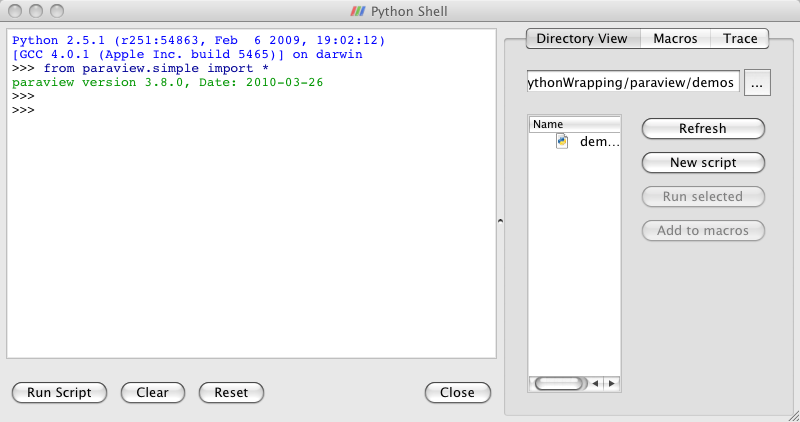
\includegraphics[width=2.5in]{images/PythonShellDialog}
\end{inlinefig}

If you are right now most interested in getting started on writing scripts,
feel free to skip to the next section past the discussion of the other ways
to invoke scripting.

ParaView comes with two command line programs that execute Python scripts:
\commandline{pvpython} and \commandline{pvbatch}.  They are similar to the
\commandline{python} executable that comes with Python distributions in
that they accept Python scripts either from the command line or from a file
and they feed the scripts to the Python interpreter.

The difference between \commandline{pvpython} and \commandline{pvbatch} is
subtle and has to do with the way they establish the visualization
service.  \commandline{pvpython} is roughly equivalent to the
\commandline{paraview} client GUI with the GUI replaced with the Python
interpreter.  It is a serial application that connects to a ParaView server
(which can be either builtin or remote).  \commandline{pvbatch} is roughly
equivalent to \commandline{pvserver} except that commands are taken from a
Python script rather than from a socket connection to a client.  It is a
parallel application that can be launch with \commandline{mpirun} (assuming
it was compiled with MPI), but it cannot connect to another server; it is
its own server.  In general, you should use \commandline{pvpython} if you
will be using the interpreter interactively and \commandline{pvbatch} if
you are running in parallel.

It is also possible to use the ParaView Python modules from programs
outside of ParaView.  This can be done by pointing the \texttt{PYTHONPATH}
environment variable to the location of the ParaView libraries and Python
modules and pointing the \texttt{LD\_LIBRARY\_PATH} (on Unix/Linux/Mac) or
\texttt{PATH} (on Windows) environment variable to the ParaView libraries.
Running the Python script this way allows you to take advantage of
third-party applications such as IDLE.  For more information on setting up
your environment, consult the ParaView Wiki.

\section{Creating a Pipeline}
\label{sec:CreatingAPipeline}

The first thing any ParaView Python script must do is load the
\textpy{paraview.simple} module.  This is done by invoking
\begin{python}
from paraview.simple import *
\end{python}
In general, this command needs to be invoked at the beginning of any
ParaView batch Python script.  This command is automatically invoked for
you when you bring up the scripting dialog in ParaView, but you must add it
yourself when using the Python interpreter in other programs (including
\commandline{pvpython} and \commandline{pvbatch}).

The \textpy{paraview.simple} module defines a function for every source,
reader, filter, and writer defined in ParaView.  The function will be the
same name as shown in the GUI menus with spaces and special characters
removed.  For example, the \pyfunc{Sphere} function corresponds to
\gui{Sources} \ra \gui{Sphere} in the GUI and the \pyfunc{PlotOverLine}
function corresponds to \gui{Filters} \ra \gui{Data Analysis} \ra \gui{Plot
  Over Line}.  Each function creates a pipeline object, which will show up
in the pipeline browser (with the exception of writers), and returns an
object that is a proxy that can be used to query and manipulate the
parameters of that pipeline object.

There are also several other functions in the \textpy{paraview.simple}
module that perform other manipulations.  For example, the pair of
functions \pyfunc{Show} and \pyfunc{Hide} turn on and off, respectively,
the visibility of a pipeline object in a view.  The \pyfunc{Render}
function causes a view to be redrawn.

\begin{exercise}{Creating and Showing a Source}
  \label{ex:CreatingAndShowingASource}%
  If you have not already done so, open the Python shell in the ParaView
  GUI by selecting \gui{Tools} \ra \gui{Python Shell} from the menu.  You
  will notice that
  \begin{python}
from paraview.simple import *
  \end{python}
  has been added for you.

  Create and show a \gui{Sphere} source by typing the following in the
  Python shell.
  \begin{python}
sphere = Sphere()
Show()
Render()
  \end{python}

  The \pyfunc{Sphere} command creates a sphere pipeline object.  Once it is
  executed you will see an item in the pipeline browser created.  We save a
  handle to the pipeline object in the variable \textpy{sphere}.  We are
  not using this variable (yet), but it is good practice to save references
  to your pipeline objects.

  The following \pyfunc{Show} command turns on visibility of this object in
  the view, and the subsequent \pyfunc{Render} causes the results to be seen.
\end{exercise}


% Chapter Batch Python Scripting
